\chapter{STP Tree Generator}
\label{stp_gen}
\section{Structure}
We split the application in three parts:
\begin{itemize}
    \item \textbf{Client}: collects STP information and sends it to the server.
        The client also handles piecing together the packets into paths.
    \item \textbf{Server}: saves the data from the clients and combines them into one tree.
    \item \textbf{Parser}: contacts the server to receive the tree and converts it into output format.
\end{itemize}
The intended form of usage is to have multiple clients in the network connecting to one server.
This naturally increases the amount of information obtainable.
STP uses only local data, which means that bridges have no knowledge of the network, except for their own port states.
Unfortunately for us, this means that it is hard to find connections between bridges.
The only way to obtain this information is to capture packets during the tree build up.
Because bridges use the default parameters they use (see Section~\ref{stp}), they will think of themselves as root.
Therefore they will propagate this information, which we can then capture.
Using the root identifier in conjunction with the message age, we can gain information about the tree structure.
An explanation of this can be found in Figures \ref{fig:build_up} and \ref{fig:information_loss}.
\begin{figure}
    \begin{centering}
        \begin{subfigure}[b]{0.4\textwidth}
            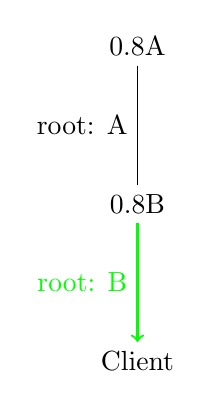
\begin{tikzpicture}
                \node (a) at (4,4) {\switch{0.8}{A}};
                \node (b) at (4,2) {\switch{0.8}{B}};
                \node (client) at (4,0) {Client};

                \draw
                (a) -- node [left] {root: A} ++ (b);

                \draw[green, thick, ->]
                (b) -- node [left] {root: B} ++ (client);

            \end{tikzpicture}
            \caption{B thinks it is root}
        \end{subfigure}
        \hspace{1cm}
        \begin{subfigure}[b]{0.4\textwidth}
            \centering
            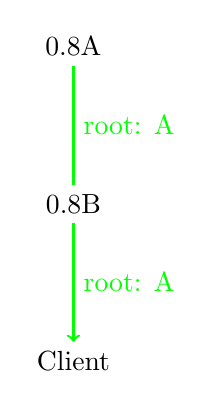
\begin{tikzpicture}
                \node (a) at (4,4) {\switch{0.8}{A}};
                \node (b) at (4,2) {\switch{0.8}{B}};
                \node (client) at (4,0) {Client};

                \draw[green, thick]
                (a) -- node [right] {root: A} ++ (b);
                \draw[green, thick, ->]
                (b) -- node [right] {root: A} ++ (client);
            \end{tikzpicture}
            \caption{Root information updated}
        \end{subfigure}
    \end{centering}
    \caption{Information gained on STP build up}
    \label{fig:build_up}
\end{figure}
\begin{figure}
    \begin{centering}
        \begin{subfigure}[b]{0.4\textwidth}
            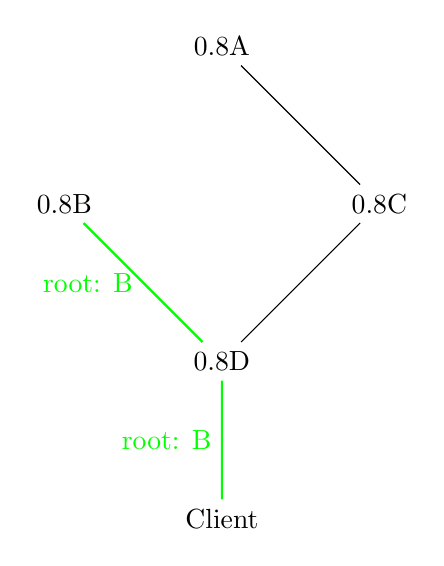
\begin{tikzpicture}
                \node (a) at (4,6) {\switch{0.8}{A}};
                \node (b) at (2,4) {\switch{0.8}{B}};
                \node (c) at (6,4) {\switch{0.8}{C}};
                \node (d) at (4,2) {\switch{0.8}{D}};
                \node (client) at (4,0) {Client};
                \draw
                (a) -- (c)
                (c) -- (d);
                \draw[green, thick]
                (b) -- node [left] {root: B} ++ (d)
                (d) -- node [left] {root: B} ++ (client);
            \end{tikzpicture}
            \caption{Some information known}
        \end{subfigure}
        \hspace{1cm}
        \begin{subfigure}[b]{0.4\textwidth}
            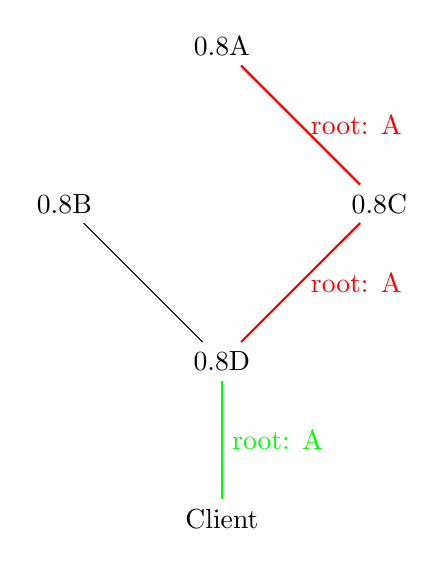
\begin{tikzpicture}
                \node (a) at (4,6) {\switch{0.8}{A}};
                \node (b) at (2,4) {\switch{0.8}{B}};
                \node (c) at (6,4) {\switch{0.8}{C}};
                \node (d) at (4,2) {\switch{0.8}{D}};
                \node (client) at (4,0) {Client};
                \draw
                (b) -- (d);
                \draw[green, thick]
                (d) -- node [right] {root: A} ++ (client);
                \draw[red, thick]
                (c) -- node [right] {root: A} ++ (d)
                (a) -- node [right] {root: A} ++ (c);
            \end{tikzpicture}
            \caption{Previous information lost}
        \end{subfigure}
        \caption{Information lost during tree build up}
    \end{centering}
\end{figure}
Unfortunately, this works only if the message age increases by one.
If any other change occurs, the client has to clear its data.
This is because in these cases we cannot guarantee that no other changes occured.
More on this can be found in the section on packet handling (Section~\ref{packet_handling}).

\section{Communication}
\section{Details}
\section{Installation \& Usage}
